\chapter{Syntax of First-Order Logic}

\emph{We now begin with the study of first-order logic. As you'll see, things will be moving a bit faster. One important thing: I assume that the ideas and methods of Part II are clear at this stage. So, we will not cover the same issues in the same level of detail as in propositional logic just for first-order logic. For example, I now assume that you know how an inductive definition works. This allows us to focus on the more interesting aspects of first-order logic.} 

\section{First-Order Languages}

	\begin{enumerate}[\thesection.1]

		\item Remember from the introduction that in first-order logic, we deal with inferences involving the \emph{quantifiers} ``for all'' and ``there exists.'' We looked at the following two examples:
		\begin{enumerate}[(1)]
		\setcounter{enumii}{2}
	
		\item This ball is scarlet and everything that's scarlet is red. So, this ball is red.
		
		\item The letter is in the left drawer. So there is something in the left drawer.
	
	\end{enumerate}
		Note that the kind of abstraction we did in propositional logic---abstracting away from concrete sentences via sentence letters---will not work in these kinds of inferences. Take (4), for example. If we abstract from the concrete sentences, we get the following argument form: 
		\[p\therefore q,\]
		where $p$ stands for ``the letter is in the left drawer'' and $q$ stands for ``there is something in the left drawer.'' Clearly, though, $p\nvDash q$ (just let $v(p)=1$ and $v(q)=0$); so, according to propositional logic, inference (4) is invalid, which is clearly absurd.
		
		The moral of the story is that in predicate logic, the \emph{internal structure} of the sentences is important. When all we care about are the sentential connectives, then abstracting sentences to sentence letters is fine; but when we care about claims, like `` there is something in the left drawer,'' then this abstraction is too coarse-grained. We need to abstract \emph{less}.
		
		\item The first step towards first-order logic is to take into account the \emph{grammatical structure} of simple sentences. A traditional way of looking at the structure (which is in essence still alive in linguistic syntax theory) is to consider the \emph{term-predicate} structure of sentences. A sentence like ``the ball is scarlet'' says of a thing, the ball, that it has a property, being red. The sentence talks about the ball via the \emph{singular term} ``the ball'' and it talks about being red using the \emph{predicate} ``\dots is red.'' Now just like we abstracted away from sentences via sentence letters  in propositional logic, in first-order logic, we abstract away from terms and predicates via \emph{term symbols} and \emph{predicate symbols}. The rationale is that just like in propositional logic the concrete sentences didn't matter for validity, in first-order logic, the concrete terms and predicates don't matter. To see this, consider the following inferences:
		\begin{enumerate}[(1')]
		\setcounter{enumii}{2}
	
		\item This train is slow and everything that's slow is yellow. So, this train is yellow.
		
		\item The dog is in the car. So there is something in the car.
	
	\end{enumerate}
Both of these inferences are valid, just like their counterparts (3) and (4). Clearly whatever  terms and predicates you fill in here, in the inferences remain valid. So, we can abstract away from them.

		\item In first-order logic, we represent terms using \emph{term symbols}, typically denoted $t,u,v,\mathellipsis.$ There are actually several different \emph{kinds} of terms. In first-order logic, we distinguish three:
		\begin{enumerate}[(i)]
		
			\item \emph{proper names}, like ``Johannes'' or ``Angela''
			
			\item \emph{pronouns}, like ``he,'' ``she,'' and ``it''
			
			\item \emph{functional terms}, like ``the birthplace of Ada Lovelace''
		
		\end{enumerate}
These classifications, just like the examples, stem from natural language. But it's fruitful to compare these categories to expressions from mathemateze that we've discussed in \S2. In mathematics, constants are proper names, variables are pronouns, and functions are \dots well \dots functions. In fact, this terminology is the very same we use for the corresponding syntactic categories in our formal language for first-order logic. The reason for this is the origin of first-order logic as the study of \emph{mathematical} reasoning. We typically use constants $a,b,c,\mathellipsis$ to abstract from proper names, we use variables $x,y,z,\mathellipsis$ to abstract from pronouns, and we use functional terms $f,g,h,\mathellipsis$ to abstract from functional expressions.

		\item It's worth thinking about functional expressions in natural language for a moment. Take the above example ``the birthplace of Ada Lovelace.'' This is a singular terms that refers to a place, namely London. The structure of the expression is that a functional expression ``the birthplace of \dots'' is applied to another term, the proper name ``Ada Lovelace.'' Correspondingly, in first-order logic, we take the structure of ``the birthplace of Ada Lovelace'' to be: \[f(a),\] where $f$ stands for ``the birthplace of \dots'' and $a$ stands for Ada Lovelace. Note that there are conditions for us to understand a natural language expression as a function: they are the conditions for function-hood we discussed in 3.6.5. The expression ``the birthplace of \dots'' expresses a function since everybody has a birthplace and no person has two birthplaces (here we're assuming that only names for people can be put in for the ``\dots''). Note that function expressions in natural language, just like in mathematics, can come with different \emph{arities}. For example, the expression ``the last common ancestor (LCA) of \dots and \underline{\phantom{\dots}}'' is a function expression in natural language that refers to the last person that both \dots and \underline{\phantom{\dots}} directly descend from. It is generally believed that for any pair of humans there is a LCA and no two people can have more than one LCA. So, the expression, ``the last common ancestor of Alan Turing and Ada Lovelace'' refers to one and only one individual, we just don't know which one. Formally, we'd write it like this: \[f(a,b),\] where $f$ stands for ``the last common ancestor (LCA) of \dots and \underline{\phantom{\dots}},'' $a$ for Alan Turning and $b$ for Ada Lovelace.
		
		Note that function expressions can be combined to make more complicated function symbols. We can talk, for example, about the ``the LCA of Ada Lovelace and the LCA of Alan Turing and Angela Merkel,'' which we'd formally write as \[f(a,f(b,c)),\] where $c$ stands for Angela Merkel. This is not really different from what happens in mathematics, when we combine mathematical operations, as in: \[(n+m)\cdot 2\]\[\exp(n+m)\]\[(a\cdot b)+(c\cdot d)\]
				
		\item In first-order logic, we represent predicates using \emph{predicate symbols}, typically $P,Q,R, \mathellipsis.$ So, the logical structure of ``the ball is scarlet'' according to first-order logic is: \[P(t),\] where $t$ stands for the ball and $P$ for the predicate ``\dots is scarlet.'' The predicate ``is scarlet'' is what's called a \emph{unary} predicate, it expresses a property of \emph{one} object. There are also predicates with higher \emph{arities}: ``\dots is in \underline{\phantom{\dots}}'' is a \emph{binary predicate} or \emph{relation symbol}; ``\dots lies between \underline{\phantom{\dots}} and \textbf{---}'' is a \emph{ternary predicate}; and so on for \emph{$n$-ary predicates}. An $n$-ary predicate expresses that a certain \emph{relation} holds between $n$ objects, each denoted by a term. So, the general form of a simple sentence in first-order logic is: \[R(t_1, \mathellipsis, t_n),\] where $R$ is an $n$-ary predicate symbol and $t_1,\mathellipsis, t_n$ are terms. The sentence ``the letter is in the left drawer,'' for example, is formalized as \[R(t, u),\] where $t$ stands for the letter, $u$ for the left drawer, and $R$ for the binary predicate ``\dots is in \underline{\phantom{\dots}}.''
		
		\item Now, the real interesting part in first-order logic are the quantifiers, they are what gives the logic its expressive strength. In first-order logic, as we already hinted at, we consider two quantifier expressions: ``for all'' and ``there exists'' (and synonymous expressions like ``every,'' ``some,'' \dots). Our inferences (3) and (4) provide examples of how these expressions are used in natural language. Let's briefly talk about how we treat them in the language of first-order logic. In first-order logic, we use the quantifiers with the help of variables to formalize general claims, like ``everything that's scarlet is red'' or ``there is something in the left drawer.'' Remember that an important role of variables in mathematics is to allow us to make general claims about mathematical objects (cf. 2.2.6 and 2.2.7). In first-order logic, the variables play the same role. Here's how. Take the claim:
		\begin{itemize}
		\item Everything that's scarlet is red.
		\end{itemize}
In first-order logic, we take the underlying logical structure of the expression to be:
	\begin{itemize}
		\item Every object is such that if it is scarlet, then it is red.
	\end{itemize} 
In any case, clearly, the two sentences are equivalent: if the one is true, the so is the other and vice versa. So, logically, they should be treated as the same. Now note that ``object,'' and ``it'' are indefinite terms, they refer to one arbitrary but fixed object. They are, essentially, variables! So, in half-formal terms, the structure of ours sentence is:
	\begin{itemize}
	
		\item Every $x$ is such that if $x$ is scarlet, then $x$ is red.
	
	\end{itemize}
We've already talked about how we abstract from predicates in first-order logic, and the ``if \dots, then \underline{\phantom{\dots}}'' is treated just like in propositional logic, so the only interesting thing is the expression ``every.'' This is where the quantifiers come in. We use the \emph{universal quantifier} $\forall$ as our abstract representation of phrases like ``every,'' ``for all,'' ``each,'' and so on. So, ultimately, the form of our example in first-order logic is \[\forall x(S(x)\to R(x)),\] where $S$ stands for the predicate ``\dots is scarlet'' and $R$ stands for ``\dots is red.'' So, putting it all together, inference (3) get's formalized as \[S(a), \forall x(S(x)\to R(x))\therefore R(a),\] where $a$ is a constant for the ball. 

	\item In order to formalize our inference (4), we need to talk about ``there exists,'' ``there is,'' ``some,'' and so on. In first-order logic, we abstractly represent these expressions by the \emph{existential quantifier} $\exists$. Otherwise, the idea is the same as in ``for all.'' So, from ``there is something in the left drawer'' we get via ``there is some object such that it is in the left drawer'' to ``there is some $x$ such that $x$ is in the left drawer,'' and finally reach \[\exists xR(x,b),\] where $R$ stands for the predicate ``\dots is in \underline{\phantom{\dots}}'' and $b$ is a constant for the left drawer. The whole inference (4) therefore becomes \[R(a,b)\therefore\exists xR(x,b),\] where additionally $a$ is a constant for the letter.

	\item Those are the basic ideas of first-order languages. To sum up, let's put our new vocabulary in a table together with names and intended reading:
	\begin{longtable}{c | l | l}
	Symbol & Name & Reading\\\hline
	$a,b,c,\mathellipsis$ & Constants & Proper names, math. constants\\
	$x,y,z,\mathellipsis$ & Variables & Pronouns, math. variables\\
	$f,g,h, \mathellipsis$ & Function symbols & Functional expressions\\
	$P,Q,R,\mathellipsis$ & Predicate symbols & Predicates, properties, relations\\
	$\forall $ & Universal quantifier & every, for all, each, \dots\\
	$\exists$ & Existential quantifier & there exists, there is, for some, \dots
	\end{longtable}
	
	We'll now make the syntax of first-order logic formally precise. At the end of the chapter, we'll talk about formalization in first-order logic.
		
	\end{enumerate}
	
\section{Terms and Formulas}

	\begin{enumerate}[\thesection.1]

		\item Remember that in order to define a formal language, $\mathcal{L}$,\footnote{In this chapter, $\mathcal{L}$ will stand for a fixed but arbitrary \emph{first-order} language.} we need to specify its vocabulary and its grammar (4.1.4). In first-order logic, it's standard to package the non-logical vocabulary together in what's called a ``signature.'' A \emph{signature} is a structure $\mathcal{S}=(\mathcal{C}, \mathcal{F}, \mathcal{R}, ar)$ such that:
		\begin{enumerate}[(i)]
		
			\item $\mathcal{C}$ is a set of \emph{constant symbols}
			
			\item $\mathcal{F}$ is a set of \emph{function symbols}
			
			\item $\mathcal{R}$ is a set of \emph{predicate symbols}
			
			\item $ar:\mathcal{F}\cup\mathcal{R}\to\mathbb{N}$ is a function that assigns to each function and predicate symbol a fixed natural number, its \emph{arity}
		\end{enumerate}
	So, a signature gives us the constants, functions, and predicates that we have available in our language $\mathcal{L}$. Additionally, via the function $ar$, the signature also tells us the arity of our function and predicate symbols, which we can't just ``read off'' the symbols. Note that just like every set of sentence letters determined a different propositional language, in first-order logic, every signature determines a different first-order language.
	
		\item Strictly speaking the arity function $ar$ is always part of the signature. However, it's a bit annoying to always have it around since its function is purely auxiliary. We'll therefore introduce the notational convention that for $R\in\mathcal{R}$, $R^n$ means that $R$ is such that $ar(R)=n$, and similarly for $f\in\mathcal{F}$, $f^n$ means that $f$ is such that $ar(f)=n$. This allows us to drop the arity function from the specification of a signature and still record all the information it provides. Note well, however, that the expression $R^n$ is \emph{not} a symbol of our language, only $R$ is. The notation $R^n$ is purely suggestive.  
	
		\item \emph{Examples}:
		
			\begin{enumerate}[(i)]
			
				\item Signature of $\mathcal{L}_{PA}$, the language of arithmetic, is \[\mathcal{S}_{PA}=(\{0\}, \{S^1, +^2, \cdot^2\}, \emptyset),\] Note that the language of arithmetic doesn't have any predicate symbols in its signature, which is perfectly fine.
				
				\item A real extreme example (!) is the \emph{empty} signature $\mathcal{S}_\emptyset=(\emptyset,\emptyset,\emptyset).$ This signature determines the language $\mathcal{L}_\emptyset$ of \emph{pure first-order logic}.
				
				\item Also set-theory can be looked at from the perspective of first-order logic. The signature of the language of set-theory $\mathcal{L}_\in$ is defined as \[\mathcal{S}_\in=(\{\emptyset\}, \emptyset, \{\in^2\}).\] It has only the binary predicate $\in$.
			
			
				\item A less concrete example: $\mathcal{S}=(\{a,b,c\}, \{f^1, g^2\}, \{P^1, R^2\})$ has three constants: $a,b,c$; two function symbols: the unary function symbol $f$ and binary function symbol $g$; and two predicate symbols: the unary $P$ and the binary $R$.
			
			\end{enumerate}
		
		In the following, we'll always assume that we're dealing with some arbitrary but fixed signature $\mathcal{S}=(\mathcal{C}, \mathcal{F}, \mathcal{R})$.
	
		\item The \emph{logical} vocabulary of every first-order language, however, is the same. It consists of:
		\begin{enumerate}[(i)]
		
			\item the set of \emph{variables}: $\mathcal{V}=\{x,y,z,\mathellipsis\}$\footnote{In the following, we shall always assume that we have a fixed set of infinitely many variables at our disposal. We don't care so much about how they are written: $u,v,w,\mathellipsis$ is equally fine as $x_1, x_2, x_3,\mathellipsis$.}
			
			\item the \emph{sentential operators}: $\neg,\land,\lor,\to,\leftrightarrow$
			
			\item the \emph{identity predicate}: $=$
			
			\item the \emph{quantifiers}: $\forall,\exists$
			
			\item the \emph{parentheses}: $(,)$.
		
		\end{enumerate}
		The only symbol in the logical vocabulary we haven't discussed so-far is the identity predicate $=$. The purpose of this symbol is relatively clear: it expresses the predicate ``\dots is identical to \underline{\phantom{\dots}}.'' ``But is it among the \emph{logical} vocabulary and not in the signature?'' you ask? Good question! This has to do with the fact that we treat identity as a distinguished, \emph{logical} concept. What this precisely means will become clear only in the next lecture. But for now you can already see one aspect of it. Remember that when we abstract natural language expressions into first-order formulas, we abstract away from the concrete predicates in question (8.1.2): `the letter is in the left drawer'' becomes $R(a,b)$. With identity, we won't play this game, identity always gets formalized as identity. So, ``the birthplace of Ada Lovelace is identical to the birthplace of Alan Turing'' get's formalized as \[f(a)=f(b),\] where $a$ stands for Ada Lovelace, $b$ for Alan Turing, and $f$ for ``the birthplace of \dots.'' Note that we don't need to say what $=$ stands for, this is clear! We'll talk about identity some more when we talk about formalization.
		
		\item Remember that above (8.1.4) we mentioned that function expressions can be \emph{nested}, i.e. used within one another. This necessitates that we give a recursive definition of the terms of our language, which is what we'll do next. The set $\mathcal{T}$ of \emph{terms} is recursively defined as the smallest set $X$ such that:
		\begin{enumerate}[(i)]
		
			\item \begin{enumerate}[(a)]
			\item $\mathcal{V}\subseteq X$
			\item $\mathcal{C}\subseteq X$
			\end{enumerate}
			\item If $t_1, \mathellipsis, t_n\in X$ and $f^n\in\mathcal{F}$, then $f(t_1, \mathellipsis, t_n)\in X$
		
		\end{enumerate}
		In words, the terms are all the variables and constants plus the functional combinations of those. 
		
		\item \emph{Examples}:
		
			\begin{enumerate}[(i)]
			
				\item In $\mathcal{S}_{PA}$, we have, for example, \[S(0),S(S(0)),\mathellipsis\in\mathcal{T}\]\[S(x), S(y), +(0,0), \cdot(0,0), \cdot (S(x), +(0,0)),\mathellipsis\in\mathcal{T}\]	
				We'll introduce some notational conventions in $\mathcal{S}_{PA}$: 
				\begin{enumerate}[(a)]
					
					\item We write ${n}$ instead of $\underbrace{S(\mathellipsis S(0)\mathellipsis)}_{n\text{ times}}$. So, for example, ${1}$ is short for $S(0)$, ${2}$ is short for $S(S(0))$, and so on. This allows us to write more natural expressions, like $\cdot ({2},{2})$, which officially is $\cdot(S(S(0)),S(S(0)))$.
					
					\item To make things even more natural, we allow ourselves to use ``infix notation'' with $+$ and $\cdot$, i.e. instead of the official $\cdot(2,4),$ we allow ourselves to write $(2\cdot 4)$. The parentheses, however, are necessary, since we want to be able to disambiguate between $((2\cdot 4)+1)$, which intuitively denotes 9, and $(2\cdot (4+1))$, which intuitively denotes 10.
				
				\end{enumerate}
			
				\item The only terms in the empty signature $\mathcal{S}_\emptyset$ are the variables $x,y,z,\mathellipsis.$
				
				\item The only terms in the signature $\mathcal{S}_\in$ are $\emptyset$ and the variables. 
				
				\item Assuming that $f^2\in\mathcal{F}$, we have \[f(x,x), f(x,y), f(y,x), f(y,y), f(f(x,y), f(y,x)),\mathellipsis\in\mathcal{T}\]
			\end{enumerate}
					
		\item Note that in our function expressions, we don't pay attention to the idea of domains and ranges we painstakingly introduced in 3.6.4: for \emph{any} term $t$ a unary function symbol $f$ generates a new term $f(t)$. It is possible, and in some cases necessary, to develop a syntax theory for terms which takes into account the domains and ranges of functions by means of \emph{typing}. This is, for example, important when we study the logical foundations of programming languages, which often make use of typing. In this course, however, we won't pay that much attention to functions, and therefore typing. Instead, we focus on the grammar of \emph{formulas}. Correspondingly, we allow ourselves the leisurely assumption that every function is defined for every object.
		
 		\item Now, after everything we've said, it should be relatively clear what the recursive syntax of $\mathcal{L}$ looks like. The set $\mathcal{L}$ of \emph{formulas} is recursively defined as the smallest set $X$ such that:
		\begin{enumerate}[(i)]
		
			\item \begin{enumerate}[(a)]
			
				\item If $R^n\in\mathcal{R}$ and $t_1, \mathellipsis, t_n\in \mathcal{T},$ then $R(t_1, \mathellipsis, t_n)\in X$.
				
				\item If $t_1,t_2\in \mathcal{T}$, then $t_1=t_2\in X$
				
				\end{enumerate}
			
			\item \begin{enumerate}[(a)]
			
				\item if $\phi\in X$, then $\neg \phi\in X$
				
				\item if $\phi,\psi\in X$, then $(\phi\circ\psi)\in X$ for $\circ=\land,\lor,\to,\leftrightarrow$
				
				\item if $\phi\in X$ and $x\in \mathcal{V}$, then $Qx\phi\in X$ for $Q=\exists,\forall$
			
			\end{enumerate}
							
		\end{enumerate}
		
		The initial elements of $X$, the formulas given by (i.a--b), are also called \emph{atomic formulas}.

		
		\item One quick notational convention. Instead of $\neg{t_1=t_2}$, we allow ourselves to write $t_1\neq t_2$.
			
			\item \emph{Examples}:
			
				\begin{enumerate}[(i)]
				
					\item Here are some formulas in $\mathcal{L}_{PA}$:
					\[x=10\]
					\[S(x)=44\]
					\[2+2=4\]
					\[1\cdot1=0\]
					\[\forall x S(x)\neq 0\]
					\[(2\cdot 2)=5\land S(44)=7)\]
					\[\forall x\forall y(x\neq y\to S(x)\neq S(y))\]
					\[\forall x\forall y(S(x)=y+1\to S(x)=S(y))\]
					\[\forall x\exists yS(x)=y\]
					
				Note that the only atomic formulas in $\mathcal{L}_{PA}$ are equations, i.e. formulas of the form $t_1=t_2$.
				
				\item Here are some formulas in $\mathcal{L}_\emptyset$:
				
				\[x=y\]
				\[(x=y\land y\neq z)\]
				\[\forall x\exists y(x=y\land \forall z y\neq z)\]
				\[\forall x\exists y x\neq y\]
				\[\exists x\exists y(x\neq y\land \forall z(z=x\lor z=y))\]
				
				\item Here are some formulas in $\mathcal{L}_\in$:
				
				\[{\in}(x,x)\]
				\[\forall x{\in}(\emptyset,x)\]
				\[\neg\exists x{\in}(x,\emptyset)\]
				\[\forall x({\in}(x,y)\to {\in}(x,z))\]
				\[\forall x\forall(x=y\leftrightarrow\forall z({\in}(z,x)\leftrightarrow {\in}(z,y))) \]			
				
				In $\mathcal{L}_\in,$ to make things more natural, we allow ourselves the notation $t\in u$ instead of the official ${\in}(t,u)$. Using this convention, the examples become:
				\[x\in x\]
				\[\forall x~\emptyset\in x\]
				\[\neg\exists x~x\in \emptyset\]
				\[\forall x(x\in y\to x\in z)\]
				\[\forall x\forall y(x=y\leftrightarrow \forall z(z\in x\leftrightarrow z\in y))\]
				This almost looks like the elementary set theory we studied in \S3. And, in fact, this is the language you use to develop \emph{formal} set-theory as a first-order theory.
				
				
				\item Finally, I shall use the abstract signature $\mathcal{S}=(\{a,b,c\}, \{f^1, g^2\}, \{P^1, R^2\})$ to give some \emph{extreme} examples:
				
				\[R(f(g(a,b)),g(f(a),f(b)))\]
				\[\forall x P(f(a))\]
				\[\forall x(P(a)\to \exists yR(x,y))\]
				\[(\forall xP(x)\land \forall xQ(x))\]
				\[\forall x(P(x)\lor \forall xQ(x))\]
				\[(P(x)\leftrightarrow \forall y\forall xR(x,y))\]
				
				All of these are perfectly fine formulas of first-order logic.
				
				\end{enumerate}

		\item How do we prove that an expression $\sigma$ is \emph{not} a formula? Well, just like in propositional logic (cf. 4.1.9). Once we've introduced parsing trees in the following section, it will, in fact, be relatively straight-forward to adopt our algorithm from 4.3.10 to first-order logic. But we shall not do this explicitly, rather it will be left as an exercise (8.9.4). More generally, in first-order logic, we shall not focus so much on the more nit-picky details of syntax, like proving that a formula is an expression or not. We have bigger fish to fry.
		
		\item Since we're not so much concerned with very detailed syntax, we can already introduce the notational conventions here. Actually, they are precisely the same as in propositional logic (cf. \S4.5). To see that we can't leave out parentheses with the quantifiers, let's quickly look at one example. In the expression $\forall x(P(x)\to S(a))$, we really cannot leave out any parentheses. If we would, we'd get $\forall xP(x)\to S(a)$, which is very different from $\forall x(P(x)\to S(a))$. To see the difference, let's interpret $P$ as the predicate ``\dots passes,'' $S$ as ``\dots is surprised,'' and $a$ as denoting me. Under this reading, $\forall xP(x)\to S(a)$ says that if everybody passes, then I'm surprised. This is true---though, I'd be positively surprised. The formula  $\forall x(P(x)\to S(a))$, instead, says that for every individual student, if that student passes, I'm surprised. This is certainly false: I believe in every single one of you \smiley
		
		\item Also the topic of proof by induction we can handle rather quickly. Since the set of formulas is defined recursively, proof by induction works just like in propositional logic: we show that all formulas have a property by showing that the atomic formulas have the property and that it's preserved under the constructions:
		 \begin{theorem}
		Let $\Phi$ be a condition on formulas. If we can show:
		\begin{enumerate}[(i)]
		
			\item  \begin{enumerate}[(a)]
			
				\item $\Phi(R(t_1,\mathellipsis, t_n))$ for all $R^n\in \mathcal{R}$ and $t_1,\mathellipsis, t_n\in\mathcal{T}$
				
				\item $\Phi(t_1=t_2)$ for $t_1,t_2\in \mathcal{T}$
			
			\end{enumerate}
			
			\item \begin{enumerate}[(a)]
			
			\item For all $\phi\in\mathcal{L}$, if $\Phi(\phi)$, then $\Phi(\neg\phi)$.

			\item For all $\phi,\psi\in\mathcal{L}$, if $\Phi(\phi)$ and $\Phi(\psi)$, then $\Phi((\phi\circ\psi))$, for $\circ=\land,\lor,\to,\leftrightarrow$.
			
			\item For all $\phi\in\mathcal{L}$, if $\Phi(\phi)$, then $\Phi(Qx\phi)$ for $Q=\forall,\exists$.

		
		\end{enumerate}
		\end{enumerate}
		Then we can conclude that for all $\phi\in\mathcal{L}$, $\Phi(\phi)$.
		\end{theorem}
		\begin{proof}
		Completely analogous to the proof of Theorem 4.2.1 (induction in propositional logic).
		\end{proof}
		
		\item Note that also the set $\mathcal{T}$ is inductively defined, so we can also prove things about terms by means of induction:
		 \begin{theorem}
		Let $\Phi$ be a condition on terms. If we can show:
		\begin{enumerate}[(i)]
		
			\item  \begin{enumerate}[(a)]
			
				\item $\Phi(a)$ for all $a\in\mathcal{C}$
				
				\item $\Phi(x)$ for all $x\in\mathcal{V}$
			
			\end{enumerate}
			
			\item If $\Phi(t_1), \mathellipsis,\Phi(t_n),$ then $\Phi(f(t_1,\mathellipsis,t_n))$.
		\end{enumerate}
		Then we can conclude that for all $t\in\mathcal{T}$, $\Phi(t)$.
		\end{theorem}
		\begin{proof}
		Just like induction over formulas.
		\end{proof}
		
	  \item Similarly, function recursion works standardly:
		the sets of terms and formulas are inductively defined, hence we can use function recursion on them.
		The pattern is the same as always: give the value for the initial elements and say how to calculate the value for more complex elements based on the values of their components.
		As an example, let's generalize the notion of complexity from propositional logic (4.4.4) to first-order logic.
		First, we define a complexity
		$c:\mathcal{T}\to\mathbb{N}$
		for terms by saying:
	\begin{enumerate}[(i)]
	
		\item \begin{enumerate}[(a)]

			\item $c(a)=0$ for all $a\in\mathcal{C}$
			
			\item $c(x)=0$ for all $x\in \mathcal{V}$
	
			\end{enumerate}
			
		\item $c(f(t_1, \mathellipsis, t_n))=max(c(t_1), \mathellipsis, c(t_n))+1$ for all $f^{n}\in\mathcal{F}$ and $t_{1}, \mathellipsis, t_{n}\in\mathcal{T}$
	
	\end{enumerate}
Using the function on terms, we define a complexity function $c:\mathcal{L}\to\mathbb{N}$ on formulas by saying:
		\begin{enumerate}[(i)]
		
			\item  \begin{enumerate}[(a)]
			
				\item $c(R(t_1,\mathellipsis, t_n))=max(c(t_1), \mathellipsis, c(t_n))$ for all $R^{n}\in\mathcal{R}$ and $t_{1}, \mathellipsis, t_{n}\in\mathcal{T}$
				
				\item $c(t_1=t_2)=max(c(t_1), c(t_2))$ for $t_{1},t_{2}\in \mathcal{T}$
			\end{enumerate}

			
			\item \begin{enumerate}[(a)]
			
			\item $c(\neg\phi)=c(\phi)+1$
			\item $c(\phi\circ\psi)=max(c(\phi),c(\psi))+1$, for $\circ=\land,\lor,\to,\leftrightarrow$.
			
			\item $c(Qx\phi)=c(\phi)+1$ for $Q=\forall,\exists$.

		
		\end{enumerate}
		\end{enumerate}
		As you can see, things work really analogously to the way they work in propositional logic.

	\end{enumerate}

\section{Parsing Trees and Occurrences}

	\begin{enumerate}[\thesection.1]

		\item In this section, we develop the notion of a parsing tree for formulas in first-order logic. Since all the constructions of propositional logic are also constructions of first-order logic, we actually just have to \emph{add} new clauses to Definition 4.3.5. Well, that's not \emph{exactly} true. Note that, in contrast to sentence letters in propositional logic, also the atomic formulas of first-order logic, like $R(a, g(x, f(a)))$, have an internal structure that we need to parse. We therefore begin by defining the notion of a parsing tree for \emph{terms}.
		
		\item We recursively define the function $T$ that assigns to each term $t\in\mathcal{T}$ its parsing tree as follows:
		
\begin{center}
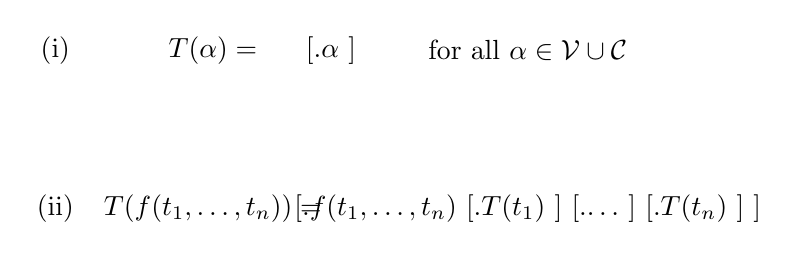
\begin{tikzpicture}
\node at (-2,1) {(i)};

\node at (0,1) {$T(\alpha)=$};
\node at (1.5,1) {\Tree [.$\alpha$ ]};
\node at (4,1) {for all $\alpha\in\mathcal{V}\cup\mathcal{C}$};

\node at (-2,-1) {(ii)};
\node at (0,-1) {$T(f(t_1, \mathellipsis,t_n))=$};
\node at (4,-1) {\Tree [.{$f(t_1, \mathellipsis,t_n)$} [.{$T(t_1)$} ] [.$\mathellipsis$ ] [.{$T(t_n)$} ] ]};

\end{tikzpicture}
\end{center}

		\item \emph{Examples}:
		
			\begin{enumerate}[(i)]
			
				\item Here's the parsing tree for the term $4=S(S(S(S(0))))$ in $\mathcal{L}_{PA}$:
				
				\begin{center}
				\Tree [.$S(S(S(S(0))))$ [.$S(S(S(0)))$ [.$S(S(0))$ [.$S(0)$ [.$0$ ] ] ] ] ]
				\end{center}
				
				\item Here's the parsing tree for $(2\cdot (2+1))=(S(S(0))\cdot (S(S(0))+S(0)))$
								
				\begin{center}
				\Tree [.$(S(S(0))\cdot (S(S(0))+S(0)))$ [.$S(S(0))$ [.$S(0)$ [.$0$ ] ] ] [.$(S(S(0))+S(0))$ [.$S(S(0))$ [.$S(0)$ [.$0$ ] ]  ] [.$S(0)$ [.$0$ ] ] ] ]
				\end{center}
				
				\item One last, more abstract example:
				
				\begin{center}
				\Tree [.{$f(g(a,b))$} [.$g(a,b)$ [.$a$ ] [.$b$ ] ] ]
				\end{center}
				
					\end{enumerate}

				
				\item We can now give the general, recursive definition of a parsing tree for a formula $\phi\in\mathcal{L}$:			
				
				\begin{center}
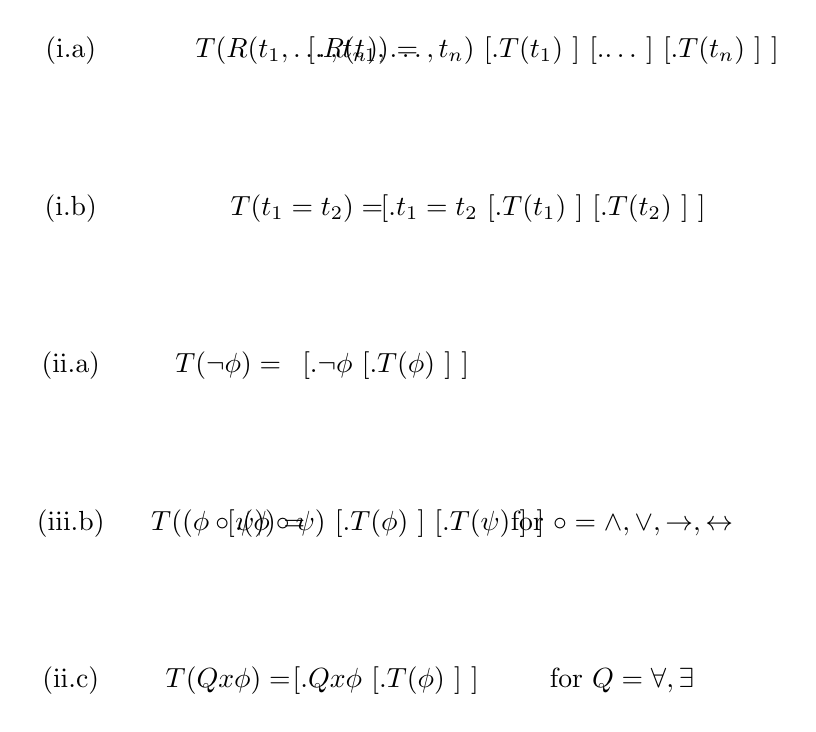
\begin{tikzpicture}
\node at (-2,1) {(i.a)};

\node at (1,1) {$T(R(t_1, \mathellipsis, t_n))=$};
\node at (4,1) {\Tree [.{$R(t_1, \mathellipsis,t_n)$} [.{$T(t_1)$} ] [.$\mathellipsis$ ] [.{$T(t_n)$} ] ]};

\node at (-2,-1) {(i.b)};
\node at (1,-1) {$T(t_1=t_2)=$};
\node at (4,-1) {\Tree [.$t_1=t_2$ [.$T(t_1)$ ] [.$T(t_2)$ ] ]};

\node at (-2,-3) {(ii.a)};
\node at (0,-3) {$T(\neg \phi)=$};
\node at (2,-3) {\Tree [.$\neg \phi$ [.$T(\phi)$ ] ]};

\node at (-2,-5) {(iii.b)};
\node at (0,-5) {$T((\phi\circ\psi))=$};
\node at (2,-5) {\Tree [.$(\phi\circ\psi)$ [.$T(\phi)$ ] [.$T(\psi)$ ] ]};
\node at (5,-5) {for $\circ=\land,\lor,\to,\leftrightarrow$};


\node at (-2,-7) {(ii.c)};
\node at (0,-7) {$T(Qx \phi)=$};
\node at (2,-7) {\Tree [.$Qx\phi$ [.$T(\phi)$ ] ]};
\node at (5,-7) {for $Q=\forall,\exists$};


\end{tikzpicture}
\end{center}
			
	
	\item \emph{Example}. Since the idea of how to do parsing trees should be clear by now, we do just one, more involved example:
	
	\begin{center}
	
	\Tree [.{$\forall x(R(x,g(f(a),f(b)))\to \exists yR(y,y))$} [.{$R(x,g(f(a),f(b)))\to \exists yR(y,y)$} [.{$R(x,g(f(a),f(b)))$} [.$x$ ] [.{$g(f(a),f(b))$} [.$f(a)$ [.$a$ ]  ] [.$f(b)$ [.$a$ ]  ] ] ] [.$\exists yR(y,y)$ [.$R(y,y)$ [.$y$ ]  [.$y$ ] ] ] ] ]
	
	\end{center}
	
	\item At this point, we simply remark that it is now a straight-forward exercise to prove a Unique Readability Theorem for terms and formulas in first-order logic along the lines of the proof we gave in 4.3.8. Stating and proving this theorem is useful exercise.
			
	\item In the following, we shall need, for technical reasons, the notion of a \emph{stripped} parsing tree. The stripped parsing tree of a formula is the result of leaving only the main operator on each node when we're doing the ordinary parsing tree. Here is an explicit, recursive definition of stripped parsing trees for terms and formulas:\\[2ex]
	
\emph{Terms}:\\[2ex]
\begin{center}
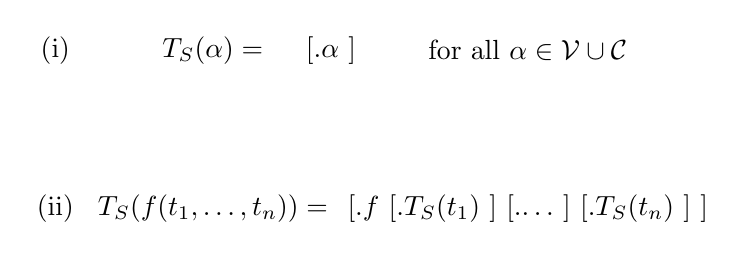
\begin{tikzpicture}
\node at (-2,1) {(i)};

\node at (0,1) {$T_S(\alpha)=$};
\node at (1.5,1) {\Tree [.$\alpha$ ]};
\node at (4,1) {for all $\alpha\in\mathcal{V}\cup\mathcal{C}$};

\node at (-2,-1) {(ii)};
\node at (0,-1) {$T_S(f(t_1, \mathellipsis,t_n))=$};
\node at (4,-1) {\Tree [.{$f$} [.{$T_S(t_1)$} ] [.$\mathellipsis$ ] [.{$T_S(t_n)$} ] ]};

\end{tikzpicture}
\end{center}	
	
\emph{Formulas}:\\[1ex]
\begin{center}
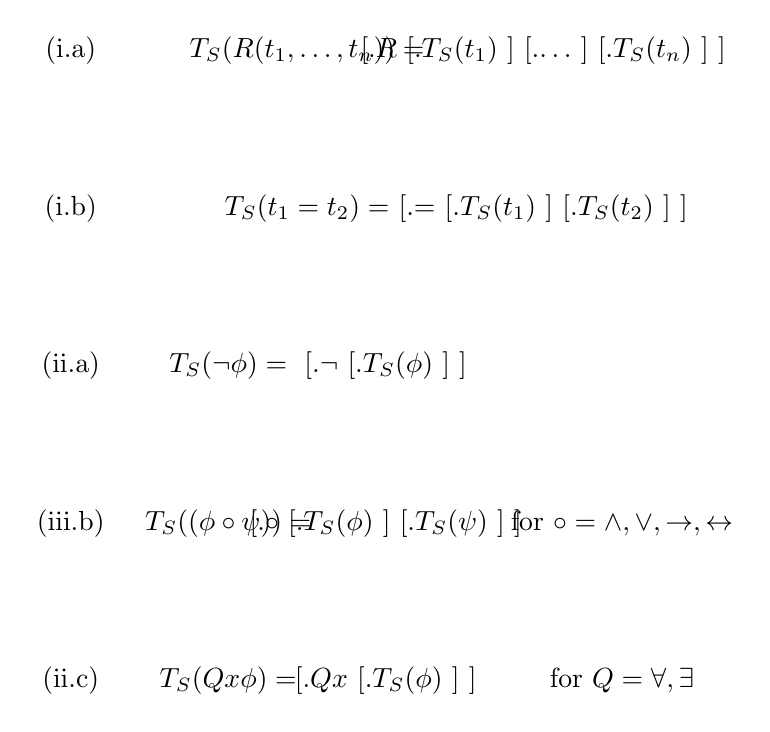
\begin{tikzpicture}
\node at (-2,1) {(i.a)};

\node at (1,1) {$T_S(R(t_1, \mathellipsis, t_n))=$};
\node at (4,1) {\Tree [.{$R$} [.{$T_S(t_1)$} ] [.$\mathellipsis$ ] [.{$T_S(t_n)$} ] ]};

\node at (-2,-1) {(i.b)};
\node at (1,-1) {$T_S(t_1=t_2)=$};
\node at (4,-1) {\Tree [.$=$ [.$T_S(t_1)$ ] [.$T_S(t_2)$ ] ]};

\node at (-2,-3) {(ii.a)};
\node at (0,-3) {$T_S(\neg \phi)=$};
\node at (2,-3) {\Tree [.$\neg$ [.$T_S(\phi)$ ] ]};

\node at (-2,-5) {(iii.b)};
\node at (0,-5) {$T_S((\phi\circ\psi))=$};
\node at (2,-5) {\Tree [.$\circ$ [.$T_S(\phi)$ ] [.$T_S(\psi)$ ] ]};
\node at (5,-5) {for $\circ=\land,\lor,\to,\leftrightarrow$};


\node at (-2,-7) {(ii.c)};
\node at (0,-7) {$T_S(Qx \phi)=$};
\node at (2,-7) {\Tree [.$Qx$ [.$T_S(\phi)$ ] ]};
\node at (5,-7) {for $Q=\forall,\exists$};


\end{tikzpicture}
\end{center}
In a sense, the information provided by the stripped parsing tree is the same as the information provided by the ordinary parsing tree: they both tell us how the formula was constructed.  In fact, it's easy to write an algorithm that translates an ordinary parsing tree into a stripped one and vice versa (exercise?). The difference between the two concepts is a difference in focus: while the ordinary parsing tree focuses on the information from which \emph{sub-formulas} a formula was constructed, the stripped parsing tree focuses on the \emph{operations} used along the way. Having easy access to this information will be useful along the way.

	\item \emph{Example}. Here's the stripped parsing tree for Example 8.3.5:
	
	\begin{center}
	
	\Tree [.{$\forall x$} [.{$\to$} [.{$R$} [.$x$ ] [.{$g$} [.$f$ [.$a$ ]  ] [.$f$ [.$a$ ]  ] ] ] [.$\exists y$ [.$R$ [.$y$ ]  [.$y$ ] ] ] ] ]
	
	\end{center}
	
	\item In the following, we shall often need to access the information provided by parsing trees. In order to be able to do so, we need to be able to refer to the nodes in a given tree in a clear fashion. For this purpose, we introduce the following (standard!) naming  conventions for nodes in trees. Let me introduce the idea by means of an example. Take the tree:
		
		\begin{center}
		\Tree [.$\bullet$ [.$\bullet$  [.$\bullet$ [.$\bullet$ ] ] [.$\bullet$ [.$\bullet$ ] [.$\bullet$ ] ] ] ]
		\end{center}
		
We then name nodes in this tree as follows:

	\begin{itemize}
	
		\item The root is always called $r$.
		
		\item The first child of the root is called $( r, 1)$.
		
		\item The first child of $( r, 1)$ is called $( r, 1, 1)$.
		
		\item The \emph{second} child of $( r, 1)$ is called $(r, 1, 2)$.
		
		\item \dots
			
	\end{itemize}
So, the nodes in our tree are: \[r, (r,1), ( r,1,1), ( r,1,2),( r,1,1, 1), ( r,1,2,1) , ( r,1,2,2).\] Note that there can be empty names for nodes. For example, the node $(r,2,1,1)$ doesn't denote a node in our tree. 

Essentially, we name a node by giving the ``directions'' for someone traveling along the edges through the nodes.\footnote{For interested: the naming of the nodes depends on how we draw the tree, but we'll ignore this complication.} Here is a more general, recursive (!) definition of the name $\ulcorner n\urcorner$ of a node $n$ in a tree:

	\begin{itemize}
	
		\item The name of the root is $r$
		
		\item The name of the $i$-th child of node $n$ is called $(\ulcorner n\urcorner, i)$.\footnote{For this too look nice, we have to ``forget'' a bunch of parentheses in $\ulcorner n\urcorner$ according to the rule $((x,y),z)=(x,y,z)$.}
	
	This definition allows you to step-by-step calculate the name of a node in a tree.
	
	\end{itemize}

	\item We shall now define the central notion of an \emph{occurrence} of an expression in a formula. Intuitively, it's pretty clear what it means for an expression to occur in a formula: an expression occurs in a formula if you need to write it down in order to write the formula. So, for example, $P(x)$ occurs in $\forall x(P(x)\lor R(x,x))$. But for our intents and purposes, this intuitive notion doesn't provide enough information. We need better access to the internal structure of the formula. We get it, via the parsing tree. First, we shall give a precise definition of the notion of an occurrence:
	
	\begin{itemize}
	
		\item An expression $\sigma$ \emph{occurs} in a term or formula $\tau$ iff $\sigma$ is the label of some node in the (ordinary or stripped) parsing tree of $\tau$.
	
	\end{itemize}

	\item Let's begin with some examples:
	
		\begin{enumerate}[(i)]	
	
	
			\item The term $S(S(0))$ occurs in the term $S(S(S(S(0))))$, since it labels the node $(r,1,1)$ in the parsing tree:
\begin{center}
				\Tree [.$S(S(S(S(0))))$ [.$S(S(S(0)))$ [.$S(S(0))$ [.$S(0)$ [.$0$ ] ] ] ] ]
				\end{center}

			\item The quantifier $\exists y$ occurs in the formula $\forall x(R(x,g(f(a),f(b)))\to \exists yR(y,y))$ since it labels the node $(r,1,2)$ in the stripped tree:
	\begin{center}
	
	\Tree [.{$\forall x$} [.{$\to$} [.{$R$} [.$x$ ] [.{$g$} [.$f$ [.$a$ ]  ] [.$f$ [.$a$ ]  ] ] ] [.$\exists y$ [.$R$ [.$y$ ]  [.$y$ ] ] ] ] ]
	
	\end{center} 


		  \item The formula
			$R(x,y)$
			occurs \emph{twice} in the formula
			$\forall x(R(x,y)\to \exists x\forall y(R(y,x)\land \neg R(x,y)))$,
			once at
			$(r,1,1)$
			and once at
			$(r,1,2,1,1,2,1)$:
\begin{center}
\begin{tabular}{c}
{\Tree [.$\forall x(R(x,y)\to \exists x\forall y(R(y,x)\land \neg R(x,y)))$
		[.$R(x,y)\to \exists x\forall y(R(y,x)\land \neg R(x,y))$ 
			[.$R(x,y)$ [.$x$ ] [.$y$ ] ]
			[.$\exists x\forall y(R(y,x)\land \neg R(x,y))$ 
				[.$\forall y(R(y,x)\land \neg R(x,y))$ 
					[.$R(y,x)\land \neg R(x,y)$ 
						[.$R(y,x)$
							[.$y$ ]
							[.$x$ ]
						]	
						[.$\neg R(x,y)$ 
							[.$R(x,y)$
								[.$x$ ]
								[.$y$ ]
							]
						]
					]
				]
			]
		]
	]
}
\end{tabular}
\end{center}

\end{enumerate}

	  \item The fact that an expression can occur more than once requires us to talk about \emph{occurrences} of expressions.
		For many purposes we want to be able to \emph{distinguish} different occurrences of expressions, we want, for example, to be able to distinguish the occurrence of
		$R(x,y)$ at $(r,1,1)$
		from the occurrence at
		$(r,1,2,1,1,2,1)$.
		We do this by defining an \emph{occurrence} of an expression in a formula as the pair $(n,\sigma)$ where $n$ is a node in the parsing tree labelled with $\sigma$.
	
	\item \emph{Examples}. Consider the formula $\forall x(R(x,y)\to \exists x\forall y(R(y,x)\land \neg R(x,y)))$. We gave the ordinary parsing tree above. Here is the stripped one:
	\begin{center}
\begin{tabular}{c}
{\Tree [.$\forall x$
		[.$\to$ 
			[.$R$ [.$x$ ] [.$y$ ] ]
			[.$\exists x$ 
				[.$\forall y$ 
					[.$\land$ 
						[.$R$
							[.$y$ ]
							[.$x$ ]
						]	
						[.$\neg$ 
							[.$R$
								[.$x$ ]
								[.$y$ ]
							]
						]
					]
				]
			]
		]
	]
}
\end{tabular}
\end{center}
	
		\begin{itemize}
		
			\item The following are all the occurrences of logical operators in the formula:
			
				\begin{longtable}{l}
					$(r,\forall x)$\\
					$((r,1),\to)$\\
					$((r,1,2),\exists x)$\\
					$((r,1,2,1),\forall y)$\\
					$((r,1,2,1,1),\land)$\\
					$((r,1,2,1,1,2),\neg)$
				\end{longtable}

				
			\item The following are all the occurrences of predicate symbols in the formula:
				
				\begin{longtable}{l}
					$((r,1,1),R)$\\
					$((r,1,2,1,1,1),R)$\\
					$((r,1,2,1,1,2,1),R)$
				\end{longtable}

			\item The following are all the occurrences of variables in the formula:
				
				\begin{longtable}{l}		
					$((r,1,1,1),x)$\\
					$((r,1,1,2),y)$\\
					$((r,1,2,1,1,1,1),y)$\\
					$((r,1,2,1,1,1,2),x)$\\
					$((r,1,2,1,1,2,1,1),x)$\\
					$((r,1,2,1,1,2,1,2),y)$
				\end{longtable}
				
				\item The following are all the occurrences of formulas in the formula:
				\begin{longtable}{l}		
					$(r,\forall x(R(x,y)\to \exists x\forall y(R(y,x)\land \neg R(x,y))))$\\
					$((r,1),(R(x,y)\to \exists x\forall y(R(y,x)\land \neg R(x,y))))$\\
					$((r,1,1),R(x,y))$\\
					$((r,1,2),\exists x\forall y(R(y,x)\land \neg R(x,y))))$\\
					$((r,1,2,1),\forall y(R(y,x)\land \neg R(x,y)))$\\
					$((r,1,2,1,1),(R(y,x)\land \neg R(x,y)))$\\
					$((r,1,2,1,1,1),R(y,x))$\\
					$((r,1,2,1,1,2),\neg R(x,y))$\\
					$((r,1,2,1,1,2,1),R(x,y))$\\
					
				\end{longtable}
				
				
			\end{itemize}

\end{enumerate}

\section{Free and Bound Variables}

	\begin{enumerate}[\thesection.1]

		%\item With the technical concepts from the previous section in place, we can now study the internal, quantificational structure of first-order formulas. We're essentially going to study how to understand first-order formulas with only the intuitive ideas laid out in 8.1 in mind.
		
		\item Variables, just like pronouns are tricky. They allow us to talk about things in general, to say things like ``everything that's scarlet is red'' in a logically precise fashion; but, at the same time, it's not always easy to figure out what your variables refer to, especially when you have more than one variable around. Take the formula $\forall x\exists yR(x,y)$, for example. If we read $R$ as ``\dots is smaller than \underline{\phantom{\dots}}'' and assume that we're only talking about numbers, then this statement says that for every number there is a number bigger than it. Now, how can you see that the ``it'' refers to the first number that we talked about and not the second? This information is encoded in the \emph{quantificational structure} of the formula: which quantifier talks about which variable. In this section, we set out to understand this structure.
		
		\item The concept that we're trying to understand is that of a quantifier \emph{capturing} a variable. The idea is as follows. Take the formula: \[\forall x(P(a)\land \neg R(x,a)).\] In this formula, the universal quantifier $\forall x$ stands at the very beginning, but clearly it ``captures'' the variable $x$ later on in the formula. So, if, for example, $a$ stands for Socrates, $P$ for ``\dots is a philosopher,'' and $R$ stands for ``\dots is a friend of \underline{\phantom{\dots}},'' then the formula should read: everybody is such that Socrates is a philosopher and they are not a friend of Socrates; or, more perspicuously, Socrates is a philosopher and nobody is his friend (\frownie). The point is this. For a quantifier to capture a variable, $x$, clearly the quantifier needs to talk about the variable, i.e. it needs to be of the form $\forall x$ or $\exists x$. But it does not need to stand immediately in front of the predicate the variable is applied to, as in $\forall xP(x)$; no, it can be farther away as in our example. 
		
		\item But is it enough for a quantifier to capture a variable that the quantifier talks about the variable and occurs before it in the formula? The answer is no. Take the formula $\forall x(\exists y \neg R(x,y)\lor (P(x)\to R(c,y)))$. Here are its ordinary and stripped parsing trees:
		\begin{center}
\begin{tabular}{ccc}
\Tree [.{$\forall x(\exists y \neg R(x,y)\lor (P(x)\to R(c,y)))$} [.{$(\exists y\neg R(x,y)\lor (P(x)\to R(c,y)))$} [.{$\exists y\neg R(x,y)$} [.{$\neg R(x,y)$} [.$R(x,y)$ [.$x$ ] [.${y}$ ] ] ] ] [.$(P(x)\to R(c,y))$ [.$P(x)$ [.$x$ ] ] [.$R(c,y)$ [.$c$ ] [.${y}$ ] ] ] ] ]

&\quad&

 \Tree [.{$\forall x$} [.$\lor$ [.{$\exists y$} [.$\neg$ [.$R$ [.${x}$ ] [.{$y$} ] ] ] ] [.$\to$ [.$P$ [.${x}$ ] ] [.$R$ [.$c$ ] [.{$y$} ] ] ] ] ]

\end{tabular}
\end{center}
In this formula, there is an occurrence of the variable $y$ at $(r,1,2,2,2)$, which is written in the formula after the quantifier $\exists y$ at $(r,1,1)$. But we should think that the quantifier does not bear the right relation to the variable since when we look at the way the formula was constructed the variable $y$ at $(r,1,2,2,2)$ wasn't even around when $\exists y$ at $(r,1,1)$ was introduced. So how could it ``capture'' the variable if it wasn't even there yet. 

A natural answer would be that a quantifier needs to be ``connected'' to the variable in the right way, i.e. by means of a path in the parsing tree. Take the occurrence of $y$ at $(r,1,1,1,1,2)$. This variable \emph{was} around when $\exists y$ at $(r,1,1)$ was introduced. In fact, we can see this by tracing a path from $y$ at $(r,1,1,1,1,2)$ to $\exists y$ at $(r,1,1)$. This gives us a second condition for a quantifier to capture a variable: in addition to the quantifier talking about the variable, there needs to be a path from the variable to the quantifier in the parsing tree. Is this enough?
	
	\item It turns out, the answer is no! This might be surprising but there is one phenomenon that we haven't properly taken into account yet. Take the formula $\forall x({N}(x)\to {\exists x}R(x,x))$. Here are the parsing trees:
\begin{center}
	
		\begin{tabular}{c c c}
	
	\Tree [.$\forall x({N}(x)\to {\exists x}R(x,x))$ [.${N}(x)\to \exists x{R(x,x)}$ [.${N}(x)$ [.$x$ ] ] [.${\exists x}R(x,x)$ [.$R(x,x)$ [.$x$ ] [.$x$ ] ] ] ] ]

	&\quad &
	
	\Tree [.$\forall x$ [.$\to$ [.${N}$ [.$x$ ] ] [.${\exists x}$ [.$R$ [.$x$ ] [.$x$ ] ] ] ] ]

	
	\end{tabular}
	\end{center}
	
	
	 If we read $N$ as ``\dots is a natural number'' and $R$ as ``\dots is smaller than or equal to \underline{\phantom{\dots}},'' then what this formula says is that for all numbers, there is a number that is smaller than or equal to itself. This statement is a bit artificial, but I hope the point is clear: the first quantifier $\forall x$ only talks about the first occurrence of $x$ at $(r,1,1,1)$. The second and third occurrence of $x$ at $(r,1,2,1,1)$ and  $(r,1,2,1,2)$ respectively, are captured by $\exists x$ at $(r,1,2)$. You can see this in the way we read the consequent of the conditional: $\exists x R(x,x)$ says that there exists a number that is smaller than or equal to itself. There is no remaining, unclear pronoun which is there for $\forall x$ to capture. This consideration gives us the final condition for a quantifier to successfully capture a variable: there cannot be another quantifier that captures the variable first. 
	
	\item Putting this all together, we get to the following official definition of a quantifier occurrence capturing or, as we typically say in logic, \emph{binding} a variable occurrence:
	
	\begin{itemize}
		
		\item Let $( n, x)$ be an occurrence of a variable $x$ in a formula $\phi$ and $( m, Qy)$ an occurrence of a quantifier $Q=\forall,\exists$ in $\phi$. Then, $( n, x)$ is {\it bound} by  $( m, Qy)$ iff
\begin{enumerate}[(i)]
\item $x=y,$
\item there is an downwards path from $m$ to $n,$
\item this path from $m$ to $n$ does not go through a node $k$ such that $( k, Q'x)$ is an occurrence of a quantifier $Q'=\forall,\exists$ in $\phi$.

\end{enumerate}
When a variable occurrence in a formula is not bound by some quantifier occurrence in the same formula, we also call the variable occurrence \emph{free}.

	\end{itemize}
	
	\item \emph{Examples}. Let's consider some examples.
	
		\begin{enumerate}[(i)]
		
			\item For the variable occurrence $((r,1,2,2,2), y)$ in $\forall x(\exists y \neg R(x,y)\lor (P(x)\to R(c,y)))$ and the quantifier occurrence $((r,1,1),\exists y)$ in the same formula, the condition (ii) is violated. For occurrence $(r,1,1,1,1,2)$, instead, we're good: $((r,1,1),\exists y)$ binds $(r,1,1,1,1,2)$. 
		
			\item We've just seen that for the variable occurrences $((r,1,2,1,1),x)$ and  $((r,1,2,1,2),x)$ in $\forall x(N(x)\to \exists xR(x,x))$, only the quantifier occurrence $((r,1,2),\exists x)$ binds them. Occurrence $(r,\forall x)$ does not bind either because condition (iii) of Definition 8.4.5 is violated. 
	
			\item The following table has the information which variable occurrence is bound by which quantifier occurrence in the formula $\forall x(R(x,y)\to \exists x\forall y(R(y,x)\land \neg R(x,y)))$ from Example 8.2.13
	
	\begin{center}
	\begin{tabular}{ c | c }
				Variable occurrence & Quantifier occurrence\\\hline
		
			$( ( r,1,1,1), x)$ & $( r, \forall x)$ \\
			$( ( r,1,2,1,1,1,1), y)$ & $( ( r,1,2,1), \forall y)$ \\
			$( ( r,1,2,1,1,1,2), x)$ & $( ( r,1,2), \exists x)$ \\
			$( ( r,1,2,1,1,2,1,1), x)$ & $( ( r,1,2), \exists x)$\\
			$( ( r,1,2,1,1,2,1,2), y)$ & $( ( r,1,2,1), \forall y)$\\
		
		\end{tabular}
		\end{center}
		
		\end{enumerate}
	
		\item Now, with the notion of variable binding in place, we can define the central concept of open and closed formulas: we say that a formula is \emph{open} iff there exists a variable occurrence in the formula that is not bound by some quantifier occurrence in the same formula. A formula is called \emph{closed} iff it's not open, i.e. iff all variable occurrences in the formula are bound by some quantifier occurrence. 
	
		\item \emph{Examples}: Let's first look at our examples:
		
		
			\begin{itemize}
			
				\item $\forall x(R(x,y)\to \exists x\forall y(R(y,x)\land \neg R(x,y)))$ is open, since $((r,1,1,2),y)$ is free.

			
				\item $\forall x(\exists y \neg R(x,y)\lor (P(x)\to R(c,y)))$ is open since $( ( r,1,2,2,2), y)$ is free
				
				\item $\forall x({N}(x)\to {\exists x}R(x,x))$ is closed.
			
			\end{itemize}

	  \item In the following, we shall study only inferences involving closed formulas or \emph{sentences} as they are typically called.
		The reason for this is that open formulas are not straight-forwardly apt to be true or false in a possible situation: an open formula, like $P(x)$, contains an unbound variable, which intuitively is something like a pronoun who's reference you don't know.
		This spells trouble for our account of valid inference.
		Suppose that somebody comes into the room and declares ``She's coming! So, we should all be happy.''
		How can you possibly determine any relation between the truth of ``she's coming'' and ``we should all be happy'' without knowing who ``she'' refers to?
		It \emph{is} possible to use free variables (and disambiguated) pronouns in a reasonable, logical way.
		For example, in mathematics, we often write an open formula
		$x+y=y+x$
		to express a general claim about all numbers, rather than using the universally quantified sentence
		$\forall x\forall y(x+y=y+x)$
		for the same purpose.
		Similarly, we reasonably reason from ``he's coming'' to ``he's not not coming;'' we don't need to know who ``he'' is for that purpose.
		But, it turns out that if we consider valid inferences between open formulas, all sort of technical difficulties pop up (they're not unsurmountable, but they're there).
		To avoid these problems, we'll focus on inferences between sentences alone.
		This is actually not that much of an restriction since we'll have to think about the truth-conditions for open formulas anyways when we try to give truth-conditions for sentences.
		Why you can already see now from a purely syntactic standpoint:
		sentences, like
		$\forall xP(x)$,
		are constructed from open formulas,
		in this case $P(x)$;
		so, if we want to trace the construction of a formula in our recursive definition of truth, we need to give the truth-conditions for the open formula
$P(x)$.
		\item It is worth, as an exercise, to prove some basic facts about free and bound variable. Here we report some propositions, leaving most of the proofs as exercises, however:
		
		\begin{proposition}
		Let $x$ be a variable and $\phi,\psi$ formulas. Then:
		\begin{enumerate}[1.]
		
			\item If $x$ occurs free in $\phi$, then $x$ occurs free in $\neg\phi$
			
			\item If $x$ occurs free in either $\phi$ or $\psi$, then $x$ occurs free in $(\phi\circ\psi)$ for $\circ=\land,\lor,\to,\leftrightarrow$
			
			\item If $x$ occurs free in $\phi$ and $y\neq x$, then $x$ occurs free in $Qy\phi$ for $Q=\forall,\exists$.
		
		\end{enumerate}
		\end{proposition}
		\begin{proof}
		We only proof 3. Suppose that $x$ occurs free in $\phi$, at $(n,x)$, and $y\neq x$. Suppose further, for contradiction, $(n,x)$ is bound by some occurrence $(k,Q'x)$ of quantifier $Q'x$, $Q'=\forall,\exists$, in $Qy\phi$. Clearly, $k$ can't be $r$, i.e. the root of the stripped parsing tree for $Qy\phi$. Why? Well, since there we find $Qy$ and by assumption $x\neq y$. So, for $(r,Qy)$, condition (i) of Definition 8.4.5 is violated, meaning $(r,Qy)$ can't violate any occurrence of $x$. But since the (stripped) parsing tree for $Qy\phi$ looks as follows, 		
		\begin{center}
		\Tree [.$Qy$ [.$T_S(\phi)$ ] ]
		\end{center}
This means that $k$ must be a node in $T_S(\phi)$. But that would mean that $(k,Q'x)$ binds $(n,x)$ in $\phi$. Contradiction. Hence $(n,x)$ is also free in $Qy\phi$, as desired.

		\end{proof}

	\end{enumerate}
	
\section{Substitution}

	\begin{enumerate}[\thesection.1]

		\item Before we talk about formalization, we will introduce the concept of \emph{substitution} of terms for (free) variables in formulas. The point of this operation is to be able, in a purely syntactic way, to specify what certain pronouns stand for. Remember that in first-order logic, we treat pronouns as variables: ``it is red,'' for example, is formalized as $R(x)$. Now, without knowing what ``it'' stands for, we cannot determine whether this sentence is true or false. In semantics, which we treat in the next chapter, we will discuss a semantic way of achieving this. But for many purposes, especially proof theory, it will be useful to be able to do this in a purely syntactic fashion, i.e. just by manipulating symbols. This is what the operation of term-substitution allows us to do. To illustrate the idea, think of the sentence ``it is red'' formalized as $R(x)$ again. Suppose further that in our language we refer to the ball using the constant $a$. A simple way of making it explicit that ``it'' stands for the ball is to replace the $x$ in $R(x)$ with $a$ to get $R(a)$, a formula that says that the ball is red. We will now define this operation as a general operation on formulas: the operation of a term substituting a term $t$ for free occurrences of a variable $x$ in a formula $\phi$. For this, we write $(\phi)[x:=t]$.
			
		\item In order to be able to define the operation, we first need to define what it means to replace a term for a variable in another term. This is because variables can be nested somewhere in functional expressions, such as $f(a, g(h(x),c))$. To handle this, we define the operation $(s)[x:=t]$ of replacing a term $t$ for a variable $x$ in another term $t$ recursively as follows:
		
			\begin{enumerate}[(i)]
			
				\item $(s)[x:=t]=\begin{cases} s & \text{if } s\neq x\\ t & \text{ if }s=x\end{cases}$ for $s\in \mathcal{C}\cup\mathcal{V}$
				
				\item $(f(t_1,\mathellipsis, t_n))[x:=t]=f((t_1)[x:=t], \mathellipsis, (t_n)[x:=t])$
			
			\end{enumerate} 
			
	Note the parentheses which indicate the \emph{scope} of the substitution operation: where to apply the operation. Let's go through one example step-by-step, let's calculate $(f(a, g(h(x),c)))[x:=c]$:
	
	\begin{align*}
	(f(a, g(h(x),c)))[x:=c]&=f((a)[x:=c], (g(h(x),c))[x:=c])\\
	&=f(a, g((h(x))[x:=c], (c)[x:=c]))\\
	&=f(a,g(h((x)[x:=c]), c)\\
	&=f(a,g(h(c),c))
	\end{align*}
Well, we could have done this without the recursive definition, sure. But the point here is that we want all of our definitions to be, at least in principle, computer implementable---and the way we can achieve this is by defining them properly, recursively.

	\item	Now we can define the notion $(\phi)[x:=t]$ of substituting $t$ for all free occurrences of $x$ in $\phi$. We do this recursively:	
		\begin{enumerate}[(i)]
	
			\item \begin{enumerate}[(a)] 
			
				\item $(R(t_1, \mathellipsis, t_n))[x:=t]=R((t_1)[x:=t], \mathellipsis, (t_n)[x:=t])$
				
				\item $(t_1=t_2)[x:=t]=t_1[x:=t]=t_2[x:=t]$
				
			\end{enumerate}
			
			\item \begin{enumerate}[(a)] 

			\item $(\neg\phi)[x:=t]=\neg((\phi)[x:=t])$

			
			\item $((\phi\circ\psi))[x:=t]=((\phi)[x:=t]\circ(\psi)[x:=t])$ for $\circ=\land,\lor,\to,\leftrightarrow$
			
			\item $(Qy\phi)[x:=t]=\begin{cases} Qy(\phi)[x:=t] & \text{if } y\neq x\\ Qy\phi & \text{if }y=x\end{cases}$ for $Q=\forall,\exists$

			\end{enumerate}
	

			\end{enumerate}
			
	The crucial clause is (ii.c), which blocks us from substituting the variable as soon as we hit upon a quantifier that binds it. This is because we only want to replace \emph{free} occurrences of variables. Why? Well, first of all, because only for free variables it's unclear what they stand for. So only for them do we need use substitution to say what they stand for. Moreover, if we replaced bound variables, we could change the meaning of statements. To see this, note that $\exists xR(x)$ says that there exists a red thing (assuming that $R$ stands for ``\dots is red''). Now, suppose that $(\exists xR(x))[x:=a]$ would yield $\exists xR(a)$. This would turn the statement ``there exists a red thing'' into the statement ``there exists an object such that the ball is red'' (assuming that $a$ stands for the ball). This is not only a weird statement, it could actually be false, even if ``there exists a red thing'' is true: suppose that the ball is blue and the cup is red. Then ``there exists a red thing'' is true but ``there exists an object such that the ball is red''  is false. \frownie
	
	\item \emph{Example}. Here is a step-by-step calculation of the result of a substitution: 
	
	$(\forall x(\exists y \neg R(x,y)\lor (P(x)\to R(c,y))))[y:=c]$
	\begin{align*}
	&=\forall x((\exists y \neg R(x,y)\lor (P(x)\to R(c,y))))[y:=c]\\
	&=\forall x(((\exists y \neg R(x,y)))[y:=c]\lor ((P(x)\to R(c,y)))[y:=c])\\
	&=\forall x((\exists y \neg R(x,y))\lor ((P(x))[y:=c]\to (R(c,y))[y:=c]))\\
	&=\forall x((\exists y \neg R(x,y))\lor (P((x)[y:=c])\to (R((c)[y:=c]), (y)[y:=c])))\\
	&=\forall x(\exists y \neg R(x,y)\lor (P(x)\to R(c,c)))
	\end{align*}
	
	%\item We conclude our discussion of substitution with a ``sanity check'' for our definition: we'll prove that if we replace a term for a variable in a formula 
	
%	\item To deepen our understanding of substitution, let's prove one characteristic proposition:
%	
%	\begin{lemma}
%	Let $x$ be a variable that occurs free in $\phi$ and $y$ any other variable. Then $y$ occurs free in $\phi[x:=y]$. 
%	\end{lemma} 
%	\begin{proof}
%	
%	
%	\end{proof}
	
	\end{enumerate}
	
\section{Formalization}

	\begin{enumerate}[\thesection.1]
	
		\item We conclude this chapter with a brief discussion of formalization in first-order logic. All the points from propositional logic still apply. The translation key in first-order logic contains the following information:
		
		\begin{enumerate}[(i)]
		
			\item A so-called \emph{domain of discourse}, $D$, which is the set of things we're talking about.
			
			\item For each constant in the signature, a natural language term it formalizes.
			
			\item For each predicate in the signature, a natural language predicate it formalizes.
			
			\item For each function symbol in the language, a natural language expression it formalizes.
			
		\end{enumerate}
	So, bottom-line, the translation key gives us the reading of the vocabulary in the signature.
	
	\item \emph{Examples}. 
	
		\begin{enumerate}[(i)]
		
		\item Here is an example of the standard translation key for $\mathcal{L}_{PA}$:
		
			\begin{itemize}
		
				\item $D=\mathbb{N}$
				
				\item $0$: the number 0
				
				\item $S$: the successor function which maps every number $n$ to the next biggest number
				
				\item $+$: addition
				
				\item $\cdot$ : multiplication
		
			\end{itemize}
			
			\item Here's a(n arbitrary) translation key for our abstract signature $\mathcal{S}=(\{a,b,c\}, \{f^1, g^2\}, \{P^1, R^2\})$:
			
			\begin{itemize}
			
				\item $D=\{x:x \text{ is a professor at UU}\}$
				
				\item $f$: the function that maps a person to their birthplace
				
				\item $g$: the function that maps two people to their LCA
				
				\item $P$: being a philosopher
				
				\item $R$ : being taller than
			
			\end{itemize}
		
		\end{enumerate}
		
		\item Here are some standard translation patterns for existential quantifiers in natural language (``some,'' ``there exists,'' \dots) using any translation key where $S$ stands for ``\dots is smart'' and $H$ stands for ``\dots is handsome.''
		
		\begin{longtable}{p{6cm} c l}
		
		Somebody who's smart exists & $\leadsto$ & $\exists x S(x)$\\

		
		There's somebody who's not smart & $\leadsto$ & $\exists x\neg S(x)$\\

Somebody's smart and somebody's handsome & $\leadsto$ & $\exists xS(x)\land \exists xH(x)$\\

Somebody's smart and handsome & $\leadsto$ & $\exists x(S(x)\land H(x))$\\
 Nobody's both smart and handsome & $\leadsto$ &$\neg\exists x(S(x)\land H(x))$\\
 
 Somebody, who's smart, is handsome & $\leadsto$ & $\exists x(S(x)\land H(x))$
		
		\end{longtable}
		
		One \emph{very important} piece of advice: what you want to say is \emph{almost never} (!): \[\exists x(S(x)\to H(x)),\] i.e. someone is such that if they're smart, then they're handsome. Remember that $\to$ is the material conditional, so this statement would already be true if there's someone who's not smart (clear? if not, read 5.1.6 again); and it's only false if there is someone who's both smart and not handsome.
		
		
		\item Here are some standard translation patterns for universal quantifiers in natural language (``for all,'' ``every,'' \dots) using the same translation key as in the previous examples:		
		\begin{longtable}{p{6cm} c l}
		
		Not everybody handsome is smart & $\leadsto$ & $\neg\forall x(H(x)\to S(x))$\\
Everybody who's smart is handsome & $\leadsto$ &$\forall x(S(x)\to H(x))$\\
A person who's smart is handsome & $\leadsto$ &$\forall x(S(x)\to H(x))$\\
Someone who's smart is handsome & $\leadsto$ &$\forall x(S(x)\to H(x))$\\
Everybody's smart and handsome & $\leadsto$ &$\forall x(S(x)\land H(x))$
		\end{longtable}
		Note well, however, that $\forall x(S(x)\land H(x))$ and $\forall x(S(x)\to H(x))$ say \emph{very} different things: the former says everybody is both smart and handsome, while the latter says that everybody who's smart is also handsome.
		
		\item Indeterminate terms, like pronouns, indexicals, etc., are formalized using free variables. Only when clearly the same thing is meant, use the same variable, if different things could be meant, use different variables:
		
		\begin{longtable}{p{7cm} c l}
		He's handsome & $\leadsto$ & $H(x)$\\
		She's handsome and smart & $\leadsto$ & $H(x)\land S(x)$\\
		He's handsome and \emph{he}'s smart & $\leadsto$ & $H(x)\land S(y)$\\
		He's handsome and she's smart & $\leadsto$ & $H(x)\land S(y)$\\
		That's a smart and handsome person & $\leadsto$ & $H(x)\land S(x)$\\
		
		
		\end{longtable}
		
		\item[8.6.5.$\frac{1}{2}$] One last piece of advice on formalization with quantifiers. If you're unsure about the quantificational structure of a sentence, it's always a good idea to follow the method we used in 8.1.6, when we introduced the quantifiers. The idea is to first rephrase a quantified statement, i.e. a statement with a quantifier expression in it, using pronouns;  to replace those pronouns with variables (following the guideline that possibly different objects get different variables); and finally to abstract the whole statement. Here's another example. Take the statement ``Every number has a successor.'' To arrive at an adequate formalization, we proceed as follows:
		\begin{itemize}
		
			\item Every number has a successor.
			
			\item Every number is such that it has a successor.
			
			\item Every object is such that if it is a number, then it has a successor.
			
			\item Every object is such that if it is a number, then there exists an object such that it's the successor of the former number.
			
			\item Every $x$ is such that if $x$ is a number, then there exists an object $y$, such that $y$ is the successor of $x$.
			
			\item $\forall x(N(x)\to \exists y(S(x)=y))$
			
			\item[] Assuming that $N$ stands for ``\dots is a number,'' and $S$ expresses the successor function.
		
		\end{itemize}
		
		\item Last, we briefly discuss how we can express that there are a fixed number of objects with a certain property. Let's suppose that we want to say that there is at least one thing that has a certain property. If we use $P$ as a predicate for a property, a simple formula that will do the trick is \[\exists xP(x)\tag{Exists$_1$}\] Now, suppose that we want to say that there is \emph{at most} one object (possibly none). How can we do that? Well, a neat little mathematical idea (that we've already used in \S2 and in the context of functions, cf. 3.6.10) is to say that to say that at most one object is so-and-so is to say that any candidate so-and-so object is \emph{unique} in being so-and-so, meaning any other object that is also so-and-so is already our object: \[\forall x\forall y(P(x)\land P(y)\to x=y)\tag{At Most$_1$}\] If we want to say that there is \emph{precisely} one object that's so-and-so, we can easily achieve this by forming the conjunction of (Exists$_1$) and (At Most$_1$):\[\exists xP(x)\land \forall x\forall y(P(x)\land P(y)\to x=y)\] This formula can be a bit simplified as follows: \[\exists x(P(x)\land \forall y(P(y)\to x=y))\tag{Exactly$_1$}\] This is, essentially, the formulation that we standardly use in mathematics to say that there is precisely one $P$.
		
		\item Ok, so far so good. Now what if we want to say that there are at least \emph{two} things that are so-and-so. Well clearly there have to be two things, $x$ and $y$ that are both so-and-so. But is this enough? Well, no! The objects $x$ and $y$ could be identical, in which case there would be only one object after all. So, we need to exclude this possibility, which gives us the following natural formula for saying that there are at least two things:
		\[\exists x\exists y(P(x)\land P(y)\land x\neq y)\tag{Exists$_2$}\]
And what about \emph{at most} two things? Well, it shouldn't be possible that there are three things, any potential third thing would have to already be one of our initial two. So, generalizing the idea from (At Most$_1$), we get: \[\forall x\forall y\forall z(P(x)\land P(y)\land P(z)\to x=y\lor x=z\lor y=z)\tag{At Most$_2$}\]
So, to say that we have \emph{exactly} two $P$'s, we can just conjoin
(Exists$_2$) and (At Most$_2$):\[\exists x\exists y(P(x)\land
  P(y)\land x\neq y)\land \forall x\forall y\forall z(P(x)\land
  P(y)\land P(z)\to x=y\lor x=z\lor y=z)\] A somewhat more palatable
formula to the same effect is: \[\exists x\exists y(P(x)\land
  P(y)\land x\neq y\land \forall z(P(z)\to x=z\lor y=z))\tag{Exactly$_2$}\]
		
		Now, you hopefully see the pattern. Can you write a formula that says that there are at least/at most/exactly 3 $P$'s?

			\end{enumerate}

%Add sections on: identity, nested quantifiers, etc.

\section{Core Ideas}

	\begin{itemize}
	
		\item In first-order logic, we take the grammatical structure of simple sentences into account.
		
		\item  Singular terms stand for objects and predicates for properties/relations.
		
		\item Quantifiers allow us talk about things in generality.
		
		\item The signature of a language consists of a set of constants, a set of function symbols, and a set of predicate symbols (the latter two with a fixed arity assignment).
		
		\item Both terms and formulas are defined inductively in first-order logic.
		
		\item We have induction for formulas and terms and function recursion.
		
		\item Parsing trees are defined for terms and functions.
		
		\item Nodes in trees have a canonical way of being named: by the directions for how to find them starting at the root. 
		
		\item Variables are bound by quantifiers.
		
		\item A formula without free variables is closed, a
                  sentence.

                  \item Substitution is a useful syntactic operation
                    that allows us to say what a variable stands for.
		
		\item Just like in propositional logic, there are guidelines for formalization.
					
	\end{itemize}

\section{Self Study Questions}

\begin{enumerate}[\thesection.1]

\item Which of the following entails that an expression is \emph{not}
  a formula of a first-order language (of appropriate signature)?

\begin{enumerate}[(a)]
\item The expression contains a sentence letter.
\item The expression contains an even number of parentheses.
\item The expression contains a symbol not from the vocabulary.
\item The expression contains a variable occurrence that is not bound
  by any quantifier occurrence.
\item The expression contains an $n$-ary function symbol followed by
  $m$-terms for $m\neq n$.
\item The expression does not have a parsing tree.
\item The expression contains quantifier occurrences that don't bind
  any variable occurrences.
\item The expression contains an odd number of parentheses.  
\item The expression contains no sentential operators.
\end{enumerate}

\item Let $\phi$ be a formula,  $(n,x)$ be a variable occurrence in
  $\phi$ and $(m,Qy)$ a quantifier occurrence in $\phi$ such that
  $(n,x)$ is bound by $(m,Qy)$. Which of the following are \emph{not}
  possible?

\begin{enumerate}[(a)]
\item $y\neq x$
\item $n=r$
\item $m=r$
\item There is a path from $m$ to $n$ such that $Qy$ is on that path
  (for $Q=\exists,\forall$)
\item There is a path from the root to $n$ which does not go through
  $m$.
\item There is a path from the root to $m$ which goes through $n$.
\item There is a path from the root to $n$ which goes through $m$.
\item There is a path from the root to $m$ which does not go through $n$.
\end{enumerate}

  \item Let $\phi$ be a formula with precisely one free variable, $x$.
	Consider the result of a substitution $(\phi)[x:=t]$ of term $t$ \emph{without free variables}
	for all free occurrences of $x$ in $\phi$.
	Which of the following can\emph{not} happen?

\begin{enumerate}
\item $(\phi)[x:=t]$ is open.
\item $(\phi)[x:=t]$ is closed.
\item $(\phi)[x:=t]$ contains no variables.
\item $(\phi)[x:=t]$ does not contain $t$.
\item $(\phi)[x:=t]$ contains free occurrences of $x$
\item $(\phi)[x:=t]$ does not contain $x$
\item $(\phi)[x:=t]$ is an atomic formula
\end{enumerate}
  
\end{enumerate}


\section{Exercises}
	
	\begin{enumerate}[\thesection.1]
	
		\item $[h]$ Define the notion of a subformula in first-order logic by generalizing Definition 4.4.2.
		
		\item $[h]$ Prove that for each formula $\phi$, if $x$ is the only variable that occurs free in $\phi$, then $Q x\phi$ is closed for $Q=\forall,\exists$.
		
		\item \begin{enumerate}[(a)]
		
		\item Use syntactic recursion to define a function $FV:\mathcal{L}\to\wp(\mathcal{V})$, which maps a formula $\phi$ to the set $FV(\phi)$ of all the variables that occur free in $\phi$.
				
		\item Prove that $FV(Qx\phi)=FV(\phi)\setminus\{x\}$ using induction on formulas.
		
		\end{enumerate}
		
		\item Adapt the algorithm from 4.3.10 to first-order logic.
		
		\item Prove 1. and 2. of 8.4.10.
		
		\item $[h]$ Is it the case that every sub-formula of a sentence is itself a sentence? If so, prove it. If not, give a counterexample.
		
		\item Let $x$ be a variable that occurs free in $\phi$ and $y$ any other variable. Is it always the case that $y$ occurs free in $\phi[x:=y]$? If so, prove it. If not, provide a counter-example.
		
		\item Do the parsing trees for  \[\forall x((R(x,x)\land \exists yR(z,y))\to \exists x\forall zB(x,x,y)).\] Determine all the occurrences of quantifiers and variables in the formula. For each occurrence of a variable determine if it's free or bound. If it's bound, determine which occurrence of a quantifier binds it.
			
		\item Step-wise calculate the results of the following substitutions.
		
		\begin{enumerate}[(i)]

			\item $[h]$ $(\forall x(R(x,y)\to\exists yR(y,y)))[y:=x]$


			\item $\forall x(P(x)\lor (\exists y(R(y,x)\to \neg Q(x)))[x:=c])$

			\item $(\forall z(R(z,z)\to (\neg R(z,z)\leftrightarrow R(z,z))))[z:=c]$

			\item  $\forall x R(x[x:=a], y[y:=b], z[x:=a])$
			
			\item  $(\forall x(\exists yR(x,y)\land \exists x\forall zR(x,z)))[x:=z]$


			\item  $(\forall x(B(x,y,y)\land \forall z(B(z,x,z)\lor \exists yB(y,y,z))))[y:=x]$


			\item  $(\forall x(R(x,x)\to (R(y,y)\lor \exists y(R(y,x)\land R(y,y)))))[y:=x]$


			\item $((\forall x\exists y(B(x,y,z))[y:=x]\lor \forall zB(z,y,x)))[y:=x]$

		\end{enumerate}
		
		\item Write down formulas in $\mathcal{L}_\in$ that say that a set $x$ has:
		
		\begin{enumerate}[(i)]
		
			\item at least 3 members
			
			\item at most 3 members
			
			\item exactly 3 members
		
		\end{enumerate}
		
		\item 
 Vertaal de onderstaande zinnen zo nauwkeurig mogelijk in de taal
van de predikatenlogica. Vergeet de vertaalsleutel niet
(discussiedomein = de verzameling der gehele getallen)
\begin{enumerate}[a.]
\item 
2 is een even getal.
\item
2 is groter dan 3.
\item $[h]$ 
De som van 2 en 3 is groter dan 4.
\item
Als dit getal groter dan 4 is, dan is het ook groter dan 3.
\item
Als dit getal niet groter dan 2 is, dan is het ook niet groter dan 3.
\item
Dit getal is kleiner dan 2 of groter dan 4.
 \end{enumerate}

\item
 Idem voor:
\begin{enumerate}[a.]
\item 
 Er is een getal groter dan 4 en er is een getal kleiner dan 4.
\item
Er is een even getal groter dan 3.
\item $[h]$ 
Ieder getal groter dan 4 is ook groter dan 3.
\item
Geen getal is groter dan 3 en kleiner dan 4.
\item
Als dit getal groter dan 4 is, dan is ieder getal dat ik hier
opgeschreven heb groter dan 4.
\item $[h]$ 
 Een getal dat kleiner dan 3 is, is kleiner dan 4.
\item
 Een getal, dat kleiner dan 3 is, is kleiner dan 4.
\item
 Er is geen getal groter dan 4 en kleiner dan 3.
 \end{enumerate}
%
\item
Idem voor:
\begin{enumerate}[a.]
\item
 Een getal dat groter is dan ieder even getal, is oneven.
\item
Ieder getal is groter dan tenminste \'e\'en getal.
\item $[h]$ 
 Er is een even getal dat kleiner is dan een oneven getal dat
groter is dan een oneven getal.
\item
 Er is geen getal dat groter is dan ieder getal.
\item
 Geen getal is groter dan zichzelf.
\item
 Ieder oneven getal is groter dan 0.
\item
 Ieder oneven getal is groter dan een even getal.
\end{enumerate}
%
\item
 Idem, maar nu met de verzameling van alle mensen als
discussiedomein, voor:
\begin{enumerate}[a.]
\item
 Wie iemand bemint, bemint zichzelf.
\item
 Wie niemand bemint, is niet verstandig.
\item
 Wie verstandig is, wordt door iemand bemind.
\item
 Iedereen bemint iemand.
\item
 Wie mij bemint, wordt door mij bemind.
\item
 Wie tegen mij is, is niet voor mij.
\item
 Wie niet voor mij is, is tegen mij.
\item
 Iedereen is \'of voor mij, \'of tegen mij.
\end{enumerate}
\item
Idem (discussiedomein = de verzameling van alle filosofen):
\begin{enumerate}[a.]
\item
 Alle filosofen publiceren in een internationaal bekend
tijdschrift.
\item
 Wie in een internationaal bekend tijdschrift publiceert en
wetenschappelijke boeken schrijft, doet hoogwaardig onderzoek.
\item
Elke filosoof die in een internationaal bekend tijdschrift
publiceert, is te verkiezen boven alle filosofen die dat niet doen.
\item
 Er is een filosoof die wetenschappelijke boeken schrijft en meer
publiceert dan allen die hoogwaardig onderzoek doen.
\item
 Voor elke filosoof die wetenschappelijke boeken schrijft geldt dat
het niet zo is dat zij/hij te verkiezen is boven alle filosofen die in
een internationaal bekend tijdschrift publiceren.
\end{enumerate}
\item $[h]$
 Gegeven is de volgende vertaalsleutel:\newline
$D$ = \{Rosja, Zebedeus, Peter\},\newline
$p$: Peter\newline
$G(x,y)$: $x$\/ is groter dan $y$\newline
$S(x,y)$: $x$\/ is sterker  dan $y$\newline
$B(x)$: $x$\/ is blij\newline
Vertaal de volgende formules naar Algemeen Beschaafd Nederlands:
\begin{enumerate}[a.]
\item
$ \exists  x\, S(x,p)$
\item
$ \forall  x\,  \forall y\, (S(x,y) \rightarrow G(y,x))$
\item
 $\forall x\, (  \exists y\, G(x,y) \rightarrow   \exists  y\, S(x,y))$
\item
 $ \lnot  \exists x\, G(p,x) \wedge   \lnot  \exists  y\, S(y,p)$
\item
 $\forall x \, (B(x) \rightarrow   \exists y\, G(y,x))$
\end{enumerate}

	\item A nice challenge at the end: give an inductive definition of a sequence of formulas $\{\phi_i\in\mathcal{L}_\empty:i\in \mathbb{N}\}$ such that $\phi_i$ says that there are precisely $i$ objects.
	
	\end{enumerate}

\vfill

\hfill \rotatebox[origin=c]{180}{
\fbox{
\begin{minipage}{0.5\linewidth}

\subsection*{Self Study Solutions}

%\emph{Some explanations in the appendix.}

\begin{enumerate}

\item[5.8.1] (a), (c), (e), (f), (h)

\item[5.8.2] (a), (b), (d), (e), (f)

\item[5.8.3] (a), (d), (e)
	
\end{enumerate}


\end{minipage}}}
	
%%% Local Variables: 
%%% mode: latex
%%% TeX-master: "../../logic.tex"
%%% End:
